\documentclass[16pt]{article}
\usepackage{graphicx}
\usepackage{amsmath} 
\usepackage[english]{babel}
\usepackage[utf8]{inputenc}
\usepackage{csquotes}
\usepackage{hyperref} 
\usepackage[margin=0.75in]{geometry}
\usepackage{apacite}
\usepackage{float}

\setlength{\parindent}{10pt}
\setlength{\parskip}{0.8em}
\renewcommand{\baselinestretch}{1.2}
\bibliographystyle{apacite}
\hypersetup{
    colorlinks=true,
    citecolor=blue,
    linkcolor=blue,
    filecolor=magenta,      
    urlcolor=blue,
}

\title{\textbf{Music, movement, development and social interaction}}

\author{Pedro de Alcantara Senra de Oliveira Neto\\ \textit{Finnish Centre of Excellence in Music,} \\ \textit{Mind, Body and Brain} }

%\date{}

\begin{document}

\maketitle

%\section{Abstract}

%Cognitive scientists have a long history of describing music in terms of its rhythmic, melodic, and harmonic properties. Recently, however, the field started to move away from strictly acoustical definitions of music, hoping that significant scientific breakthroughs could be produced if we started to see it as a multimodal phenomenon. A particularly prosperous project of multimodal investigation is that of \textbf{music and movement}. Here we explore this line of research, and we propose a series of studies to investigate how 1) music-induced movement is manifested throughout different stages of human development, and 2) how it may be affected by social variables.

%Imbued with such definitions, humanity has come a long way in understandig how it is created, produced and perceived, both from a behavioral and from a neurophisiological perspective CITAR.

\section{Background}

\subsection{The origins of music, movement, and social interaction}

Countless debates have been drawn around the issue of music, dance, and its possible evolutionary roles \cite<for a recent discussion, see>{savage2021music, mehr2021origins}\footnote{Here we use the term "dance" as a reference to any sort of music-induced movement.}. Some hypothesize, for instance, that moving to sound is disadvantageous for survival, as it can cause physical injuries, it demands high levels of caloric expenditure, and it can even capture the attention of hostile forces \cite{christensen2017not}. A more common view, however, is that dance has evolutionary benefits, and several hypothesis have been developed to investigate this idea \cite{christensen2016affective, phillips2009meaning, savage2021music}.

One of the most prominent hypothesis states that dance evolved as a mechanism of social bonding between members of a group \cite<e.g.>{savage2021music}\footnote{Other prominent hypotheses state that dancing to music provide mating and communication benefits, as well as a combination of them \cite{savage2021music}}. This view is often based on the fact that interpersonal synchronization to music is widely observed in social activities such as choirs, armies, and religious ceremonies \cite<e.g.>{huron2001music}. Recent studies generally strentgthen the social hypothesis, suggesting that group-synchronization to music can be linked to behaviors that are beneficial to society, such as collaboration \cite<e.g.>{wiltermuth2009synchrony, kirschner2010joint}, trust \cite{launay2013synchronization}, and empathy \cite{keller2014rhythm} amongst group members \cite<although, see>{kirschner2010joint}.

Beyond its apparent social benefits, music-induced movement appears to be an innate human capacity, rather than an arbitrary cultural imperative. Significan evidence suggests, for instance, that individuals as young as 5 months old tend to move when there is music \cite{zentner2010rhythmic, ilari2015rhythmic}. The same is true for older individuals \cite<e.g.>{kohn2016moving, gonzalez2020analysis}. Importantly, newborns are generally sensitive to isochronous auditory stimuli \cite{winkler2009newborn}, an ability that may be fundamental for the development of rhitmic responses to music. Finally, the idea of dance as an innate predisposition is strengthened by studies on different animal species, which show that some parrots and primates spontaneously synchronize their bodies to periodic auditory stimuli \cite< for discussions, see>{fitch2013rhythmic, patel2014evolutionary, wilson2016rhythmic}. 

%since 14 month-old infants are more likely to colaborate with an experimenter after they have bounced together to a rhythmic auditory stimulus (Cirelli et al., 2014). This particular study is relevant because it suggests that the social benefits of moving to music emerge seamlessly, with no requirement for much - if any - rational appraisal.

%At later developmental stages, adults tend to exhibit increased micro sways of the head as a response to rhythmic auditory stimuli, even if they are explicitly asked not to move (Gonzalez-Sanchez, 2018, 2020).

%Furthermore, dance seems to be a universal human activity (Nettl, 2000), which can be traced back to societies living 9 to 40 thousand years before present (Garfinkel, 1998; christensen2016affective). 
In light of these studies, it seems convinging that some aspects of music-induced movement are beneficial to group cohesion, and also that these benefits constitute the product of some innate human capacities. Still, our knowledge about developmental and social dynamics of dance is relativelly scarce. Previous investigations of music and movement did target different age-groups in different social setups, but only from a multitude of perspectives, methods and theoretical backgrounds \cite<e.g., >{launay2013synchronization, wiltermuth2009synchrony, zentner2010rhythmic, gonzalez2020analysis}. In the next section, we explore a unified framework for investigating social and developmental variables related to music-induced movement.

%Whether or not music is a privilege of humanity, its evolutionary values are still eliciting heated debates. In most cases, the role of social boding is TOP. We still do not know, however, RQ2: How does collective entrainment depend on multimodal information presence, interaction type, and group size? 

\subsection{A case for studying metrical hierarchies}

%So far, we have highlighted research questions 1 and 2, but only from a general perspective. Here we propose a series of studies designed to target these questions through a set of precisely defined auxiliary ones. Finally, we argue that finding an answer to these questions may provide us with deep insights about where music came from, what are its evolutionary values, and how it can be used as a tool to improve human life. 

The fact that individuals synchronize body-parts to periodic stimuli is nothing but a small portion of all the intricacies related to sound-movement interaction. Different from other animals \cite{fitch2013rhythmic, richter2016don}, human beings seem to be the only ones who are capable of moving in accordance with distinct \textbf{hyerarchical layers} of a pulse. Practically, this means that individuals can synchronize their bodies to different isochronous subdivisions of the same beat \cite{toiviainen2010embodied, phillips2005feeling, burger2012relationships}. In \hyperref[fig:fig1]{Figure 1}, for instance, individuals can either dance to a binary (\hyperref[fig:fig1]{Figure 1a}), or to a ternary metric hierarchy (\hyperref[fig:fig1]{Figure 1b}).

Hierarchical organizations of pitch and time are often thought to be a fundamental principle which determines how music is created, processed and perceived \cite<e.g.,>{jackendoff2006capacity}. For instance, the famous theory of tonal hierarchies \cite{krumhansl2010theory} explains why the same musical note can elicit different perceptual and phisiological responses \cite<e.g.,>{koelsch2013processing}. Not unlike tonal hierarchies, the concept of metrical hierarchies generally help us understand how different temporal patterns of acoustic stimuli elicit phisiological responses in the brain \cite{winkler2009newborn}, perceptual states \cite{desain2003formation} and, body-movement \cite{toiviainen2010embodied, burger2018synchronization}.

%We know, to date, that movement patterns can determine how individuals perceive ambiguous metrical structures, and that this effect is true for adults (CITAR), as well as for infants (Phillips-Silver \& Trainor, 2005). FALAR O QUE MAIS SE SABE. 

% Chartrand and Bargh (1999) showed that humans tend to subconsciously mimic others during social interactions,
% how we perceive music, in that vestibular stimulation caused by head movement can influence the way we perceive hierarchical rhythmic structure (meter) in music (Phillips-Silver \&  Trainor, 2008). 

%Important as it may be, we still do not know how metric hierarchies can influence music-induced movement throughout the course of human development. It is possible, for instance, that synchronizing to a pulse is an innate human capacity, but that synchronizing to different hierarchical levels is a learned ability. Conversely, it could be the case that hierarchical processing is fundamental for the development of cognitive faculties related to music, in which case hierarchy-informed movement should be an innate human capacity. 

Temporal hyerarchies offer an outstanding oportunity for studying how music-induced movement can be influenced by social variables. That is because when a given stimulus has 2 or more possible metrical interpretations (i.e., metrical ambiguity), groups of people can make the implicit choice of agreeing or not about the subdivision to which they will synchronize. If dance is, in fact, an evolutionary tool which optimizes social interaction, it might be the case that individuals are sensitive to the way that their peers move to a particular stimulus.

\begin{figure}
\centering
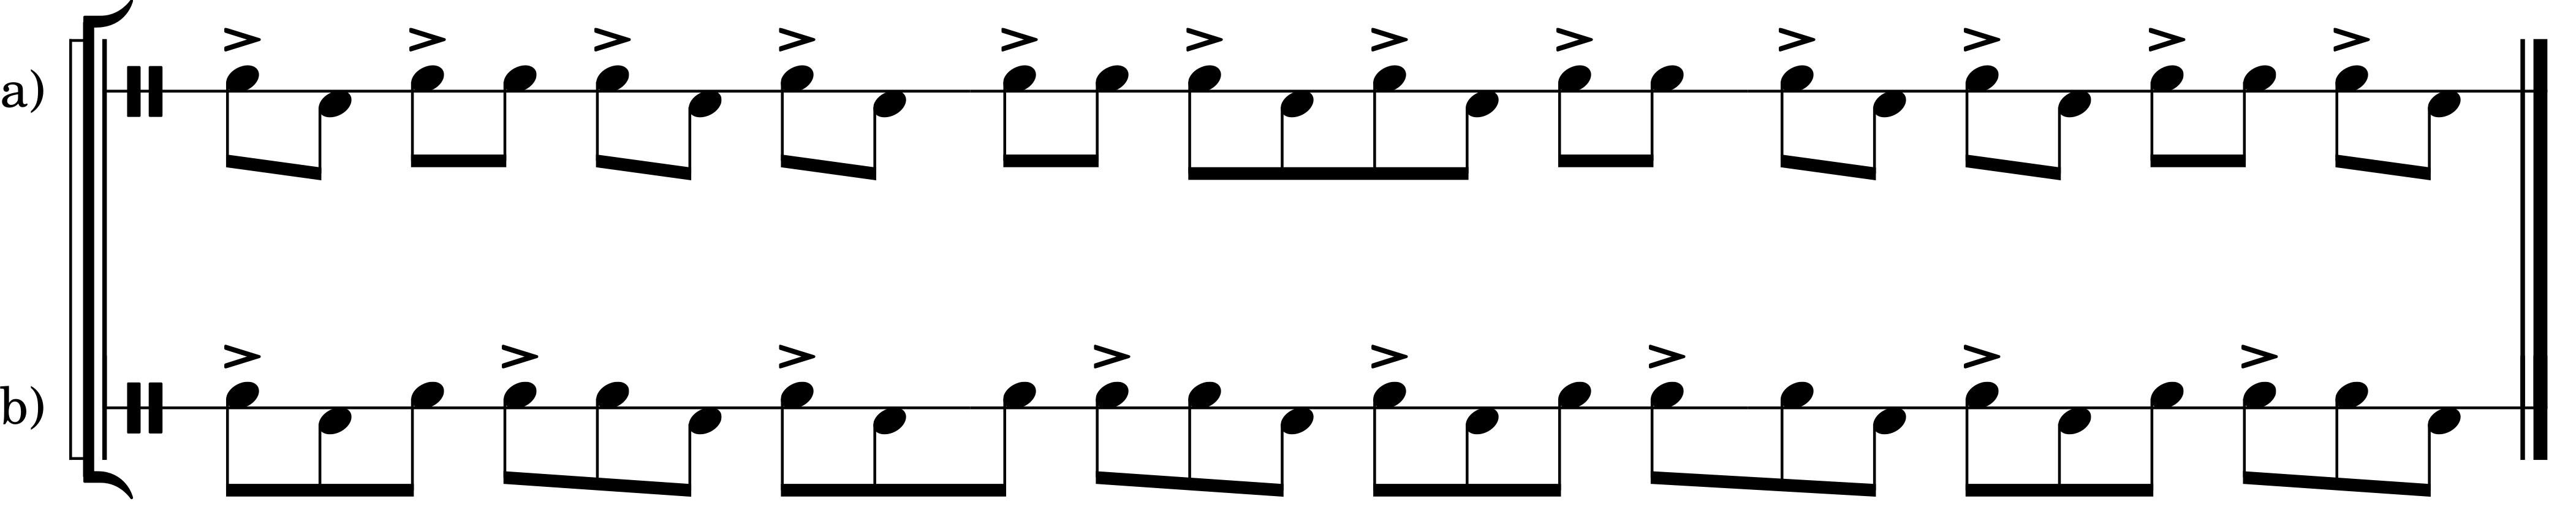
\includegraphics[scale=0.8]{ambiguous.png}
\caption{Example of metric ambiguity.}
\label{fig:fig1}
\end{figure}

%and higher levels of group-cohesion would entail higher levels of agreement about how to move to polymetric stimuli.

%in comparison with beat synchronization, moving in accordance with different metrical levels is a highly complex task, which requires CONTINUAR. Whereas we know that human-beings are generally sensitive to metrical hierarchies, we do not know how it may influence dance. It could be the case, for instance, that moving to different metric levels comes seamlessly, not unlike beat synchronization. Conversely, switching body movements between different metric layers might be an ability which is acquired throughout the course of human development. 

From the perspective of human development, metric hierarchies can also inform us about how individuals develop social abilities. It could be the case, for instance, that group-synchronization disambiguates metrical hierarchies, but only for adults and seniors. This could indicate that individuals learn to use music in social settings. Conversely, we may find that this form of social exchange is present regardless of age, which would reinforce the idea of music as an innate tool for social-bonding. Next, we propose a set of 3 studies to test these hypotheses.

%IDEIA TOP: Silent disco. One person ambiguous, others in a clear meter. Does this one person disambiguates towards what others are doing?

% We argue that this study can help us answer deep theoretical and general question, such as \textit{what are the evolutionary origins of music?}, but also more specific ones, such as 1) is the integration between music and movement innate?; 2) how does music and movement develop throughout the course of human life?; 3) how does music and movement interact with other dimensions
% Integrating movement into the study of music is often justified upon the idea that, for the majority of human history, sounds could not be disassociated from its source - a drumming rhythm could only be heard if someone's hands produced it\footnote{This is not true today, because technology allowed us to produce sounds without explicitly using the body}. However, even if movement was associated with the production of sound, it could still be the case that these activities represent related, but fundamentally separable phenomenons. \section{Research questions, methods and design} We propose a set of 3 studies, which will be administered to X participants ranging from z to Y years old. These studies will leveragethe concept of metrical hierarchies to help us understand how social and developmental variables can influence complex music-induced movement. Specifically, we will target the following questions:

%\begin{itemize}
%  \setlength\itemsep{0em}
%  \item \textbf{RQ1} Can individuals synchronize to different metric levels at the same time?
%  \item \textbf{RQ2} When in a group, are individuals more likely to chose one metric level over the other?
%  \item \textbf{RQ3} How do different sensory modalities influence group synchronization to music?
%  \item \textbf{RQ4} What acoustic variables determine group synchronization to metrically ambiguous stimuli?
%  \item \textbf{RQ5} Is interpersonal synchronization to different metrical levels a good index of group-cohesion? 
%  \item \textbf{RQ6} How does age and group-size influence the questions above? 
%\end{itemize}

\section{Action plan}

\subsection{Study design}
Studies 1, 2 and 3 are designed to evaluate how social and developmental variables interact with metric complexity. All the procedures described below will be applied to a total of 1000 participants, randing from 5 to 90 years of age. Metrical hyerarchies will be explicitly manipulated to induce 2 different pulses (i.e., binary or ternary \hyperref[fig:fig1]{Figure 1}).

\textbf{STUDY 1.} Participants, will be asked to dance freely to metrically ambiguous music \cite{phillips2005feeling, phillips2007hearing}, either in a group or in an alone condition. Auditory stimuli will be delivered through headphones (silent-disco paradigm), allowing us to bias the stimulus towards one of its two metrical hyerarchies (e.g., \hyperref[fig:fig1]{Figure 1}), but only for a subset of the participants. We hypothesize that movements from the unbiased group will reflect the metric level suggested to the biased group. This would indicate that social interaction can determine how individuals perceive metrical hierarchies.

\textbf{STUDY 2.} Similar to study 1, participants will listen to metrically ambiguous strimuli through headphones (\hyperref[fig:fig2]{Figure 2}). However, rather than dancing freely to music, participants will be blindfolded and asked to dance while holding hands in a circle (haptic coupling). A recent study by \citeA{chauvigne2019multi} has shown that, in comparison with visual and auditory modalities, haptic coupling had the strongest effect in group-synchronization. Here we expand on this study by evaluating how tactile information can disambiguate metrical hierarchies.

\textbf{STUDY 3.} This study targets the development of novel and open-access tools which will fuel ecologically valid research on music-induced movement. The proponent of this project will continue the development of an application which collects movement data from built-in accelerometers in mobile phones. As both proof-of-concept and research extension, the alone condition of study 1 will be replicated remotely, and participants will be asked to download the application and hold their phones while moving to the musical stimuli. We hypothesize that accelerometer data will convey suficient information about participant's music-induced movements, and that therefore it can be used as a tool to enable large-scale, fast, low-cost, and ecologically valid research on music and dance.

\begin{figure}[H]
\centering
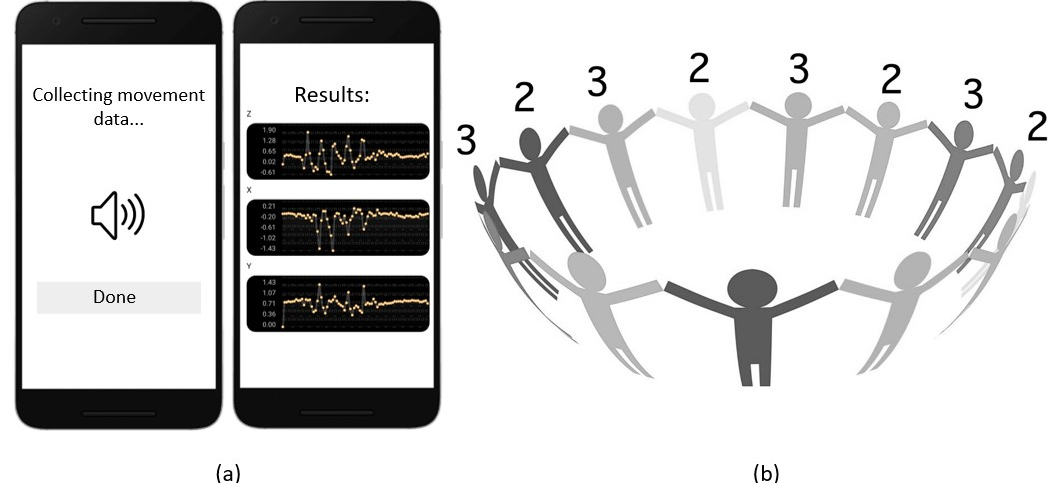
\includegraphics[scale=0.6]{design.png}
\caption{Illustratons of \textbf{(a)} accelerometer application for study 3, and \textbf{(b)} experimental design for study 2, where numbers indicate the metrical structure being administered individually to participants.}
\label{fig:fig2}
\end{figure}

\subsection{Methods}

In studies 1 an 2, data will be collected with a 15-camera Qualisys optical motion capture system. Additionally, study 3 will use built-in accelerometers in participant's mobile phones. Movement data will be analysed with cutting-edge methods such as multiset cross-spectral techniques \cite{burger2013mocap} and recurrent neural networks. Acoustic variables such as beat clarity and spectral flux, which have been shown to influence how individuals synchronize to different metrical layers \cite<e.g.>{toiviainen2010embodied, burger2018synchronization} will be extrated using MIR toolbox \cite{lartillot2007matlab}. Study 3 will extend the functionality of pre-existing technologies, such as JsPsych, \cite{de2016psychophysics}, a JavaScript library which allows researchers to collect data online and in the browser, and MoCap Toolbox \cite{burger2013mocap}.

\section{Significance of the work}

This project is part of the Finnish Centre of Excellence in \textbf{Music, Mind, Body and Brain} (MMBB), led by Professor Petri Toiviainen from the Department of Music, Art and Culture Studies (University of Jyväskylä). The MMBB adopts a multidisciplinary empirical approach that combines cognitive musicology, psychology, education, therapy, computer science, and cognitive neuroscience to determine how experiences of music change 1) over the course of human life; 2) in different developmental disorders; and 3) in different social settings. From an applied perspective, the MMBB investigates how music-based interventions can be optimized to enhance learning, emotional, cognitive, motor and social wellbeing.

As part of that research initiative, the present proposal focuses on a specific gap of knowledge identifyed by the MMBB, which concerns the dynamics of social interaction and development related to music-induced movement. As stated in the main MMBB research proposal:

\begin{displayquote}
Although evolutionary theories of music often emphasize its social origins and key role in group cohesion, bonding, and prosociality [...] the majority of music research focuses on individuals or dyads, covers only simple musical behaviours, and is limited to artificial experimental and laboratory settings. Therefore, our real-life understanding is very limited and rudimentary regarding the dynamics of and the variability in how music is used to coordinate movements and interact socially; how these functions evolve and are affected throughout different developmental stages. 
\end{displayquote}

Our proposed studies are significant because they address the issue of how multimodal and interpersonal interactions drive musical behavior in different social and developmental settings. Further, study 3 was specifically designed to overcome curent limitations of ecological validity, which are inherent to most of the previous investigations about music-induced movement. Overall, the outcomes of this project have the pottential to clarify deep issues regarding the origines of music behavior, its social functions, and how it developt throughout the course of human life.

\section{Current stage}

This project is on its early states of development, and we are currently working on the details of experiments 1 and 2, as well as on a prototype of the application proposed in study 3, which is available at \citeA{neto2022accel}. A comprehensive timetable for this study is displayed in the next section.

\section{Timetable}

The work that we propose here will be accomplished throughout the next 3 years of full-time work. The figure below represents an overview of our envisioned timetable.

\begin{figure}[h]
  \centering
  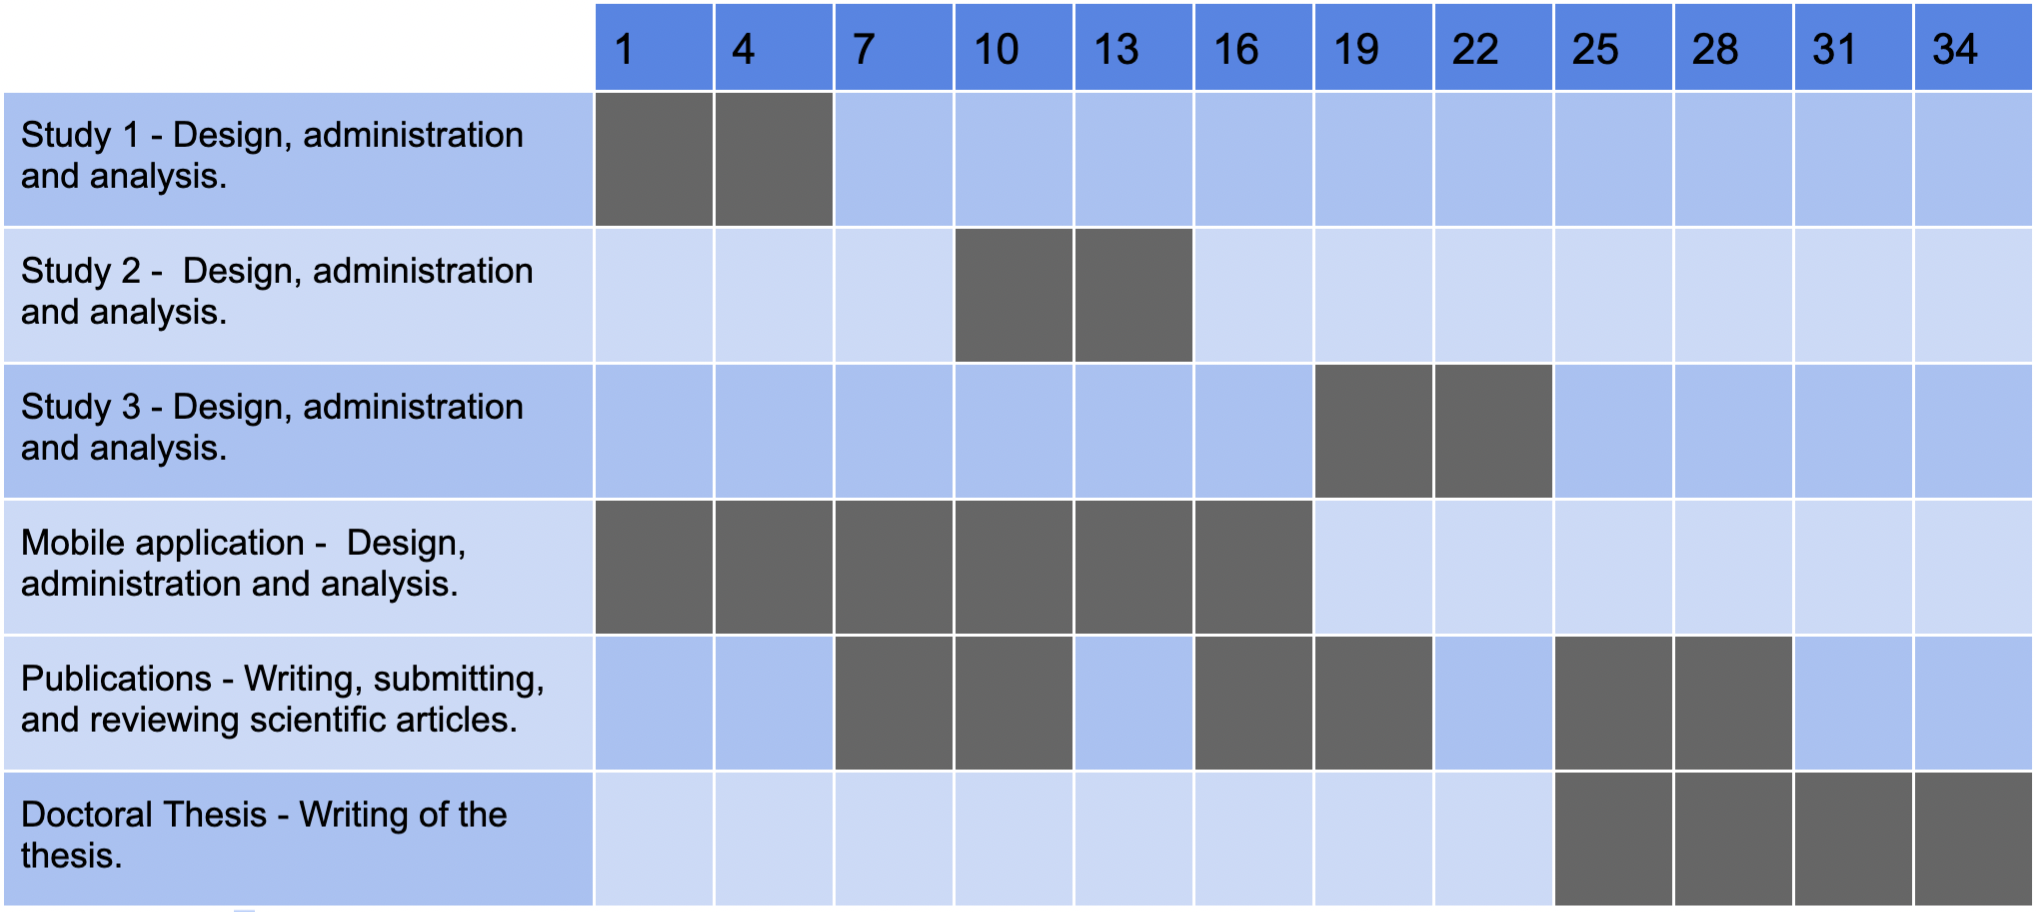
\includegraphics[scale=0.45]{images/timetable.png}
  \caption{Timetable. Each column indicates 3 months of full-time work, and the dashed line represents the current stage of our project.}
\label{fig:fig3}
\end{figure}

%\section{Study 1: variance across age groups in full-body rhythmic entrainment.}
%\section{Study 2a and group size on imitation}

%In light of its perenity alongside human societies, as well as its strong effects in social behavior, the interaction of music and dance might help  

%Experiments:
%- Prisioner's dillema after dancing alone or in group

%(Meu texto) Dance has been hypothesized to fullfill the need for comunication between large groups of human beings (Dunbar - interview). DESCRIBE WHY. Although theoretically sound, our understanding about the dynamics of interpersonal coordination in response to music is fairly limited.  WHAT DONT WE KNOW?

%(Dunbar interview: https://www.abc.net.au/radionational/programs/scienceshow/the-role-of-singing-and-dancing-in-human-evolution/7220576)

%- some songs are polymetric, meaning that their hierarchical structure of tempo can be interpreted acording to at least two distinct meters. 
%- body movement could synchronize to either;


%- problem: metric would need to REALLY be polymetric, with no favored interpretation of one metric over the other.

%Experiment:

%What is stronger? Music or visual input of peers? 

%- Experiment: 5 people dancing with 1 song, 1 person dancing different song. Does this one guy sync to others more? More speed if other song is faster? Or just type of movement, in different periods?

%- Social movement determines music perception? 

%- Given a emiole song, does the group tend toward one interpretation over the other? Essentially, here we evaluate the influence of social and visual interference with the audio signal 

%- how does age influence this?

\bibliography{./M335.bib}

\end{document}
